[12~v\textsuperscript{o}]
\`{a} l'unit\'{e};
et ces sont les logarithmes des nombres absolus, qui se trouuent calculez dans les tables.
Mais si \edtext{vous ostez les}{\lemma{vous}\Bfootnote{\textit{(1)}\ les \textit{(2)}\ ostez les \textit{L}}}
Logarithmes Tabulaires
\edtext{ou portions Hyperboliques susdites de la plus grande de toutes}{\lemma{ou}\Bfootnote{\textit{(1)}\ espaces susdits du plus grand de tous \textit{(2)}\ portions [...] toutes, \textit{L}}},
$\displaystyle QPEFQ.$ ou du logarithme du plus grand nombre, 
\edtext{$\displaystyle AE$, ou du logarithme de l'espace tout}{\lemma{$\displaystyle AE$, ou}\Bfootnote{\textit{(1)}\ de l'espace tout \textit{(2)}\ du logarithme [...] tout \textit{L}}}
entier qui est \`{a} parcourir, vous aurez les
\edtext{Logarithmes renversez}{\lemma{Logarithmes}\Bfootnote{\textit{(1)}\ de nostre proposition \textit{(2)}\ renversez, \textit{L}}},
egaux \edtext{aux portions Hyperboliques residues}{\lemma{aux}\Bfootnote{\textit{(1)}\ espaces residus \textit{(2)}\ portions Hyperboliques residues \textit{L}}}
$\displaystyle FEBDF.$ $\displaystyle FE(B)(D)F$
\edtext{etc. Donc}{\lemma{etc.}\Bfootnote{\textit{(1)}\ et \textit{(2)}\  Donc \textit{L}}}
pour calculer l\`{a} dessus il faut faire ainsi.
Essayez en combien de temps l'espace $\displaystyle EP$ est parcouru par le mobile;
ce qui sera le logarithme de dix,
supposons $\displaystyle AP$ egale \`{a} 1.
et $\displaystyle AE$ egale \`{a} 10.
et ce temps estant distribu\'{e} en 10,000,000
\edtext{parties. Pour s\c{c}avoir en combien de temps les autres espaces comme $\displaystyle BP.$ $\displaystyle (B)P$ seront parcourus, vous chercherez dans la table le nombre qui represente}{\lemma{parties.}\Bfootnote{\textit{(1)}\ Les autres espaces $\displaystyle BP.$ $\displaystyle (B)P$  \textit{(a)}\ iront parcourus  \textit{(b)}\ dont les  \textit{(c)}\ seront representez par  \textit{(aa)}\ les  \textit{(bb)}\ la \textit{(2)}\ Pour [...] vous  \textit{(a)}\ cherchez  \textit{(b)}\ chercherez  \textit{(aa)}\ le logarithme du  \textit{(bb)}\ dans la [...] represente \textit{L}}}
l'espace $\displaystyle BA.$ $\displaystyle (B)A$ et le
\edtext{temps qui doit estre}{\lemma{temps}\Bfootnote{\textit{(1)}\ qui appartient \`{a} chaque espace \textit{(2)}\ qui doit estre \textit{L}}}
employ\'{e} \`{a} parcourir chaque espace $\displaystyle BP.$ $\displaystyle (B)P$
sera design\'{e} par le logarithme de ce nombre,
c'est \`{a} \edtext{[dire]}{\lemma{}\Bfootnote{dire \textit{erg. Hrsg.}}}
l'espace $\displaystyle BP$ sera parcouru en autant de parties du temps que le logarithme
\edtext{dit, dont le temps dans lequel}{\lemma{dit,}\Bfootnote{\textit{(1)}\ telles que le temps dont \textit{(2)}\ dont [...] lequel \textit{L}}}
\pend
\newpage
\pstart \noindent
l'espace qui est comme 10, s\c{c}avoir $\displaystyle AE$, doit estre
\edtext{parcouru, contient}{\lemma{parcouru,}\Bfootnote{\textit{(1)}\ en \textit{(2)}\  contient \textit{L}}}
10,000,000. Il est \`{a} propos pour la facilit\'{e} du calcul de prendre $\displaystyle AP$, aussi petite que l'on peut
\edtext{commodement}{\lemma{commodement}\Cfootnote{Darauf folgt unmittelbar N. 34\textsubscript{4}.}} [\textit{Text bricht ab.}]
\pend
%\newpage
\pstart
\vspace{3mm}
\noindent
[\textit{Am Rand, \setline{6}ohne unmittelbar erkennbaren Zusammenhang mit dem Text:}]
\\
    \begin{wrapfigure}{l}{0.54\textwidth} 
    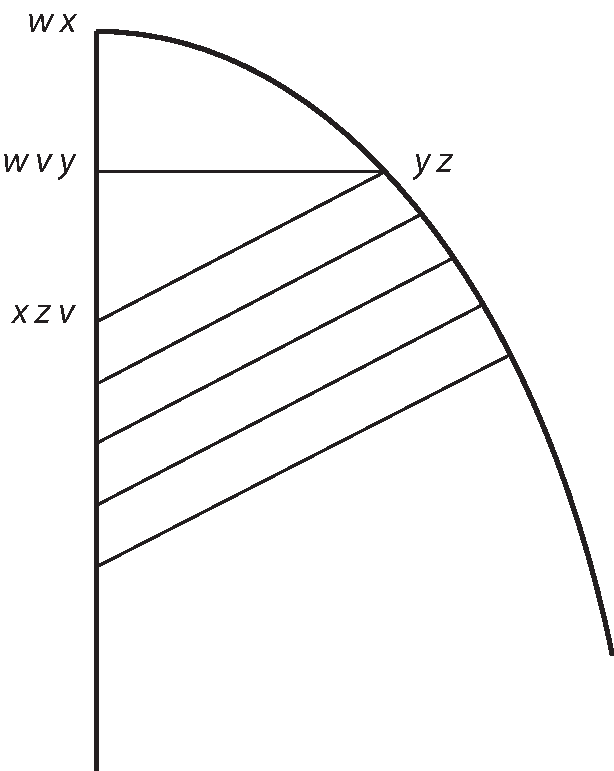
\includegraphics[trim = 0mm -6mm -45mm 0mm, clip, width=0.54\textwidth]{images/lh0350911_012v_1-d1.pdf}
    \\
    \centering
  \hspace*{-10mm}
    [\textit{Fig. 1}] % \caption{Bildbeschreibung}
    \end{wrapfigure}
%\hspace*{7,5mm}
\\[1pt]
[\textit{Neben der Zeichnung:}] \setline{5}
\\ \\
%\\
%\hspace*{65mm} 
Logarithmica obliqua.\\ \\ \\[1pt]
[\textit{Unter der Zeichnung:}] \setline{7}\\ 
\rule[-4mm]{0mm}{10mm} $\displaystyle z \, \sqcap \, a^x$\\ 
\rule[-4mm]{0mm}{10mm} $\displaystyle v \, \sqcap \frac{b}{a} z$\\ 
\rule[-4mm]{0mm}{10mm} $\displaystyle x \, \sqcap \, w + \frac{b}{a} z$\\ 
\rule[-4mm]{0mm}{10mm} $\displaystyle y \, \sqcap \, z \smallfrown \sqrt{\vphantom{\mathstrut \frac{b-a}{a}}} \frac{b-a}{a}$\\ 
\rule[-4mm]{0mm}{10mm} Ergo $\displaystyle z \, \sqcap \, y \, \sqrt{\vphantom{\mathstrut \frac{a}{a-b}}} \! \frac{a}{a-b}$.\\ 
\rule[-4mm]{0mm}{10mm} Ergo $\displaystyle x \, \sqcap \, w + \frac{b}{a} \sqrt{\frac{a}{a-b}} \ y$.\\ 
\rule[-4mm]{0mm}{10mm} Adeoque $\displaystyle y\, \, \ovalbox{$\! \displaystyle\sqrt{\vphantom{\mathstrut \frac{a}{a-b}}} \! \frac{a}{a-b} \!$} \ \sqcap \, \frac{\displaystyle a^{\scriptstyle w \, + \frac{\scriptstyle b}{\scriptstyle a} \sqrt{\frac{\scriptstyle a}{\scriptstyle a-b}} \, \scriptstyle y}}{\displaystyle\sqrt{\vphantom{\mathstrut \frac{a}{a-b}}} \! \frac{a}{a-b}}$.
%\rule[-4mm]{0mm}{10mm} Adeoque $\displaystyle y \, \ovalbox{$\! \sqrt{\vphantom{\mathstrut \frac{a}{a-b}}} \! \frac{a}{a-b} \!$} \ \sqcap \, \frac{a^{w \, + \frac{b}{a} \sqrt{\frac{a}{a-b}} \, y}}{\sqrt{\vphantom{\mathstrut \frac{a}{a-b}}} \! \frac{a}{a-b}}$.
\pend
\count\Bfootins=1500
\count\Cfootins=1500
\count\Afootins=1500
\newpage